\section{Two Higgs Doublet Model Parameters}\label{sec:2HDM}

This section summarises the work done in collaboration with Rachid Benbrik and Souad Semlali, 
for which my supervisor Stefano Moretti is also co-author~\cite{benbrik2020mapping}.
The work extends existing scan of the 2HDM model,
to locate parameter space of interest now, and after
a planned luminosity and energy upgrade to the LHC.

Five new particles are offered in the 2HDM,
two CP even (\(h\) and \(H\), with, conventionally, \(m_h < m_H\)),
one CP odd (\(A\))
and a pair of charged (\(H^\pm\)) Higgs bosons.
These come about from the addition of two complex scalar doublets \(\Phi_{1,2}\) from \(SU(2)_L\) with 
the most general gauge invariant renormalisable scalar potential given by:
\begin{align}\nonumber
V(\Phi_1,\Phi_2) =& m_{11}^2\Phi_1^\dagger\Phi_1+m_{22}^2\Phi_2^\dagger\Phi_2-[m_{12}^2\Phi_1^\dagger\Phi_2+{\rm h.c.}] \nonumber
\end{align}
\begin{align}
+& \frac{\lambda_1}{2}(\Phi_1^\dagger\Phi_1)^2
+\frac{\lambda_2}{2}(\Phi_2^\dagger\Phi_2)^2
+\lambda_3(\Phi_1^\dagger\Phi_1)(\Phi_2^\dagger\Phi_2)\nonumber\\
+&\lambda_4(\Phi_1^\dagger\Phi_2)(\Phi_2^\dagger\Phi_1) 
+\frac{1}{2}[\lambda_5~(\Phi_1^\dagger\Phi_2)^2 +~{\rm h.c.}]\nonumber\\
+&\big[ (\lambda_6(\Phi_1^\dagger\Phi_1)
+\lambda_7(\Phi_2^\dagger\Phi_2))
\Phi_1^\dagger\Phi_2+{\rm h.c.}\big] \,. \label{pot1}
\end{align}
Following the hermiticity of the scalar potential, \(m_{11}^2\), \(m_{22}^2\) and \(\lambda_{1,\ldots4}\) are real parameters
whereas \(m_{12}^2\), \(\lambda_{5,6,7}\) can be complex.
Assuming the CP-conserving version of the 2HDM, \(m_{12}^2\), \(\lambda_{5,6,7}\) and the VEVs of the fields \(\Phi_i\) are real parameters.
As a consequence of extending the discrete \(Z_2\) symmetry to the Yukawa sector in order to avoid Flavour Changing Neutral Currents (FCNCs) at tree level,
\(\lambda_{6,7}=0\), whereas the mass term \(m_{12}^2\) breaks the symmetry in a soft way.

Amongst the many signals that these additional Higgs states could produce,
of particular relevance are those involving their cascade decays,
wherein a heavier Higgs state decays in a pair of lighter ones or else into a light Higgs state and a gauge boson.
This is the case as the former process gives access to the shape of the Higgs potential of the enlarged Higgs sector
while the latter channel is intimately related to the underlying gauge structure, which may well be larger than the SM one. 
Parameter areas of interest for the process \(pp\to H\to ZA\to l^+l^-b\bar b\)
and its mirror image \(pp\to A \to ZH\to l^+l^-b\bar{b}\) 
can be established by eliminating areas ruled out by theory constraints,
previous observations and experimental sensitivity requirements.


The pattern of Branching Ratios (BRs) of the two decays \(A\to ZH\) and \(H\to ZA\) was first discussed in Refs.~\cite{Moretti1994belowThreshold} and~\cite{Djouadi1995twoAndthree}
(albeit in a Supersymmetric version of the 2HDM) and more recently implemented in Refs.~\cite{Djouadi1998HDECAY,Krause20202HDECAY} in the 2HDM.
As for production channels, the by far most relevant one  is gluon-gluon fusion, i.e., \(gg\to A\) or \(H\),
with an {occasional} competing contribution from \(b\bar b\to A\) or \(H\), respectively. 

LHC searches for the complete channels \(gg,b\bar b\to A\to ZH\) and \(gg, b\bar b\to H\to ZA\) have been carried out at both ATLAS~\cite{Aaboud2018AZHbbll} and CMS ~\cite{Khachatryan2016resonancesbbtautau,Sirunyan2020newneutral},
by exploiting leptonic decays of the gauge boson, \(Z\to l^+l^-\) (\(l=e,\mu\)),  and hadronic decays of
the accompanying neutral Higgs state, in particular, \(H\) or \(A\to b\bar b\) or \(\tau^+\tau^-\).
Based on this approach, 
current experimental data exclude heavy neutral Higgses with masses up to about \(600\)--\(700\) GeV,
depending on the BSM Higgs spectrum and the value of \(\tan(\beta)\), 
the ratio of the Vacuum Expectation Values (VEVs) of the aforementioned two Higgs doublets.
These findings are broadly in line with previous phenomenological results obtained in 
Ref.~\cite{Coleppa2014ExoticHZA}, which had forecast the LHC scope in accessing both \(A\to ZH\) and \(H\to ZA\) decays in a variety of final states. 

Here, we consider the final state \( l^+l^- b\bar b\) and start from the results of~\cite{Aaboud2018AZHbbll}
for the \(A\to ZH\) decay in order to obtain the corresponding ones for the complementary channel \(H\to ZA\),
and extend the analysis to higher energy and luminosity from planned detector upgrades.


The different transformations of the quark fields under the \(Z_2\) symmetry lead to four structures of Higgs-fermions interactions:
in Type-I only one doublet couples to all fermions;
in Type-II one of the doublets couples to the up quarks while the other doublets couples to the down quark;
in Type-X (or Lepton specific)  one of the doublets couples to all quarks and the other couples to all leptons;
in Type-Y (or Flipped) one of the doublet couples to up-type quarks and to leptons and the other couples to down-type quarks. 
\subsection{Scan}
In this study, we identify the lightest CP-even Higgs boson of the 2HDM as the observed Higgs state at the LHC, with $m_h=125$ GeV, 
and assume \(\sin (\beta-\alpha) = 1\).

We scan over the following parameter range:
\begin{equation}
\begin{gathered}
     m_{h} = 125~\text{GeV},~\sin(\beta-\alpha)=1, 0 < m_{12}^2 < 2\times 10^5~{\rm GeV},\\
     130 {\rm GeV} < m_X < 700~\text{GeV},~m_X \geq m_Y + 100~\text{GeV},\\
     m_X, m_Y~\text{chosen at}~10~\text{GeV intervals.}\\
     \tan(\beta)\in
         \begin{cases}
             \{1,~2,~3\}, & \text{if Lepton Specific}\\
             \{1,~5,~10,~20\}, & \text{otherwise}\\
         \end{cases}\\
\label{eq1}
\end{gathered}
\end{equation}
The set of values chosen for \(\tan(\beta)\), and the masses, align with the choices in~\cite{Aaboud2018AZHbbll}.
\begin{itemize}
    \item[\textbullet] For the process mediated by \AZH, we choose \(m_X~= m_A\), \(m_Y~= m_H\)  and \(m_{H^\pm} = m_A\). (Note that this choice is consistent with Ref.~\cite{Aaboud2018AZHbbll}.)
    \item[\textbullet] For the process mediated by \HZA, we choose \(m_X~= m_H\), \(m_Y~= m_A\)  and \(m_{H^\pm} = m_H\). (Note this choice is specular to that in Ref.~\cite{Aaboud2018AZHbbll}.) 
\end{itemize}


While an evident symmetry exists between the two cases, neither the constraints affecting the two processes nor their  sensitivity reaches should expected to be.
On the one hand, the role played by the heavy CP-even and CP-odd Higgs states of the 2HDM in both theoretical and experimental limits is different, owing to their different quantum numbers (and hence couplings).
On the other hand, their production and decay rates at the LHC are different despite leading to the same final states, including residual differences due to width effects entering their normalisation (but, as mentioned, not their kinematics), since, e.g., the $A$ state does not decay to $W^+W^-$ and $ZZ$ pairs while the $H$ state does and, conversely, the $A$ state decays to $Zh$ while the $H$ state does not.  
However, in the alignment limit used here these decay channels are closed.
\subsubsection{Theoretical constraints}
Within these ranges there are several theoretical and experimental constraints for the parameter points of the 2HDM to pass, discussed below.	
\begin{itemize}
	\item Unitarity: various scattering processes  require that unitarity is conserved at the tree-level at high energy.
    The unitarity requirements in the 2HDM have been studied in~\cite{Kanemura1993LeeQuiggThacker, Akeroyd2000TreeLevel, arhrib2000unitarity}.
	Sets of eigenvalues $e_i$ ($i-1, ... 12$) for the scattering  matrix of all Higgs and Goldstone bosons of the 2HDM are obtained as follows:
	\begin{eqnarray}
	&& e_{1,2} =  \lambda_3+2\lambda_4\pm 3 | \lambda_5| , \quad  \quad  e_{3,4} = \lambda_3\pm\lambda_4 , \quad e_{5,6} =  \lambda_3\pm|\lambda_5|,  \nonumber \\
	&&
	e_{7,8} = 3(\lambda_1+\lambda_2)\pm\sqrt{9(\lambda_1-\lambda_2)^2+4(2\lambda_3+\lambda_4|)^2},  \nonumber \\
	&&
	e_{9,10} = \lambda_1+\lambda_2\pm\sqrt{(\lambda_1-\lambda_2)^2+4|\lambda_5|^2},  \nonumber \\
	&&
	e_{11,12}  = \lambda_1+\lambda_2\pm\sqrt{(\lambda_1-\lambda_2)^2+4|\lambda_5|^2}.
	\end{eqnarray}
    We require all \(e_i\)'s to be less than 16\(\pi\) for each \(i=1,...12\).
\item Perturbativity constraints \cite{Kanemura1993LeeQuiggThacker,Branco_2HDMreview2011} implies that all that the quartic couplings of the scalar potential satisfy the condition \(|\lambda_i| \leqslant 8 \pi\) for each \(i=1,...5\).
	
	\item Vacuum stability requires the scalar potential to be bounded from below~\cite{Gunion2003decouple} by satisfying the following inequalities:
	\begin{eqnarray}
	\lambda_{1,2}>0,  \,\,
	\lambda_3>- \sqrt{\lambda_1\lambda_2}, \,\,
	\lambda_3+\lambda_4-|\lambda_5|> - \sqrt{\lambda_1\lambda_2}.~~~
	\end{eqnarray}
	
\end{itemize}
In practice the theoretical constraints are automatically checked by the program 2HDMC~\cite{Eriksson20102HDMC}.
The program will tell us if a selected parameter combination is valid,
however owing to the range of possible values in \(m_{12}^2\) some level of curve fitting to the valid points
is required to augment the MC sampling.
Points that satisfy the most constraints are fitted to a polynomial and
values of \(m_{12}^2\) near the surface of the polynomial is samples further.
The objective is to locate values that are permitted by all theory constraints.

\subsubsection{Experimental constraints}
In addition to theoretical constraints experimental constrains need to be accounted for.
\begin{itemize}
	\item EW Precision Observables (EWPOs) \cite{Haller2018EWUpdate}, such as the oblique parameters $S$ and $T$ \cite{Peskin:1991sw, Grimus2008Oblique}, require a level of degeneracy between the charged Higgs boson state and one of the heavier neutral Higgs bosons. Here, we assume $m_{H^\pm} = m_{A}$  or $m_H$, as appropriate (see below), so that the $T$ parameter exactly vanishes in the alignment limit. 
    \item Exclusion limits at 95\% Confidence Level (CL) from Higgs searches at colliders (LEP, Tevatron and LHC) via HiggsBounds, version 5.3.2~\cite{Bechtle2009higgsbounds, Bechtle2011higgsbounds2, Bechtle2014higgsbounds4} are enforced.
    Furthermore, the ATLAS Collaboration has set an upper limit at 95\% CL on the production cross section $\sigma$ of the $A$ state times its decay BR into $ZH\to l^+l^-b\bar b$, i.e., \(\sigma(A)\times {\rm BR}(A\rightarrow ZH \rightarrow l^+l^-b\bar b)\)~\cite{Aaboud2018AZHbbll}, that is not included in this tool, hence we have accounted for it separately.
	
\item Constraints from the Higgs boson signal strength measurements are automatically satisfied as we assume $\sin(\beta-\alpha) =1$.	
	
\item Constraints of {flavour physics observables,} namely, \(B \rightarrow X_s \gamma,~ B_{s,d} \rightarrow \mu^+\mu^-\) and \(\Delta m_{s,d}\)~\cite{Haller2018EWUpdate}.		
\end{itemize}

Comparing to observed and expected exclusion limits requires obtaining branching ratios and production cross sections.
The relevant branching ratios, \AZH{}, \HZA{}, \Abb{} and \Hbb{} are calculated with 2HDMC~\cite{Eriksson20102HDMC}.
The production cross sections of the heavy CP-even ($H$) and CP-odd ($A$) Higgs bosons,
at Next-to-Next-to-Leading Order (NNLO) in QCD, 
for both $gg\to H,A$ and $b\bar b\to A,H$, at the Centre-of-Mass (CM) energies of 13 TeV and 14 TeV,
are calculated using SusHi~\cite{Harlander2013SusHi, Harlander2017Bento, Harlander2002nexttonext, Harlander:2003ai}. 

2HDMC code also includes an interface to HiggsBounds, which is used to apply the aforementioned exclusion limits at 95\% CL from Higgs searches at LEP, Tevatron and LHC.

The choice of \(m^2_{12} = m_A^2 \tan(\beta) / (1 + \tan(\beta))^2\) enables us to reconstruct the exclusion limits at 95\%  CL given in Ref~\cite{Aaboud2018AZHbbll}.
However, this choice does not actually allow to satisfy theoretical constraints in all four types of 2HDM.

The first part of this study deals with the two production and decay processes \(pp \rightarrow H(A) \rightarrow ZA(H)\rightarrow b\overline{b}l^{-}l^{+}\).
The observed and expected confidence limits for all four types of Yukawa couplings in the 2HDM are produced at \(\sqrt{s}=13\)~TeV, with an integrated luminosity, $L$, of \(36.1~{\rm fb}^{-1}\),
by combining our calculations with the data from Ref.~\cite{Aaboud2018AZHbbll}. 
In the second part, we rescale the expected exclusion limit to the CM energy of \(\sqrt{s}=14\)~TeV,
with an integrated luminosity of \(300~{\rm fb}^{-1}\), by calculating the so called `upgrade factor' for both signals and backgrounds, while retaining the acceptance and selection efficiencies of the analysis at the lower $\sqrt s$ value. The change in energy will naturally affect signals and backgrounds differently. We treat the former by using SusHi (as intimated) and the latter by  using {MadGraph5, version 2.6.4}~\cite{alwall_madgraph2011}. (For completeness, the
 background is considered to be any reducible or irreducible SM process that creates a pair of $b$-jets plus a pair of electrons or muons, as in Ref.~\cite{Aaboud2018AZHbbll}.)

\subsection{Numerical results}


\begin{figure}[t!]
	\centering
    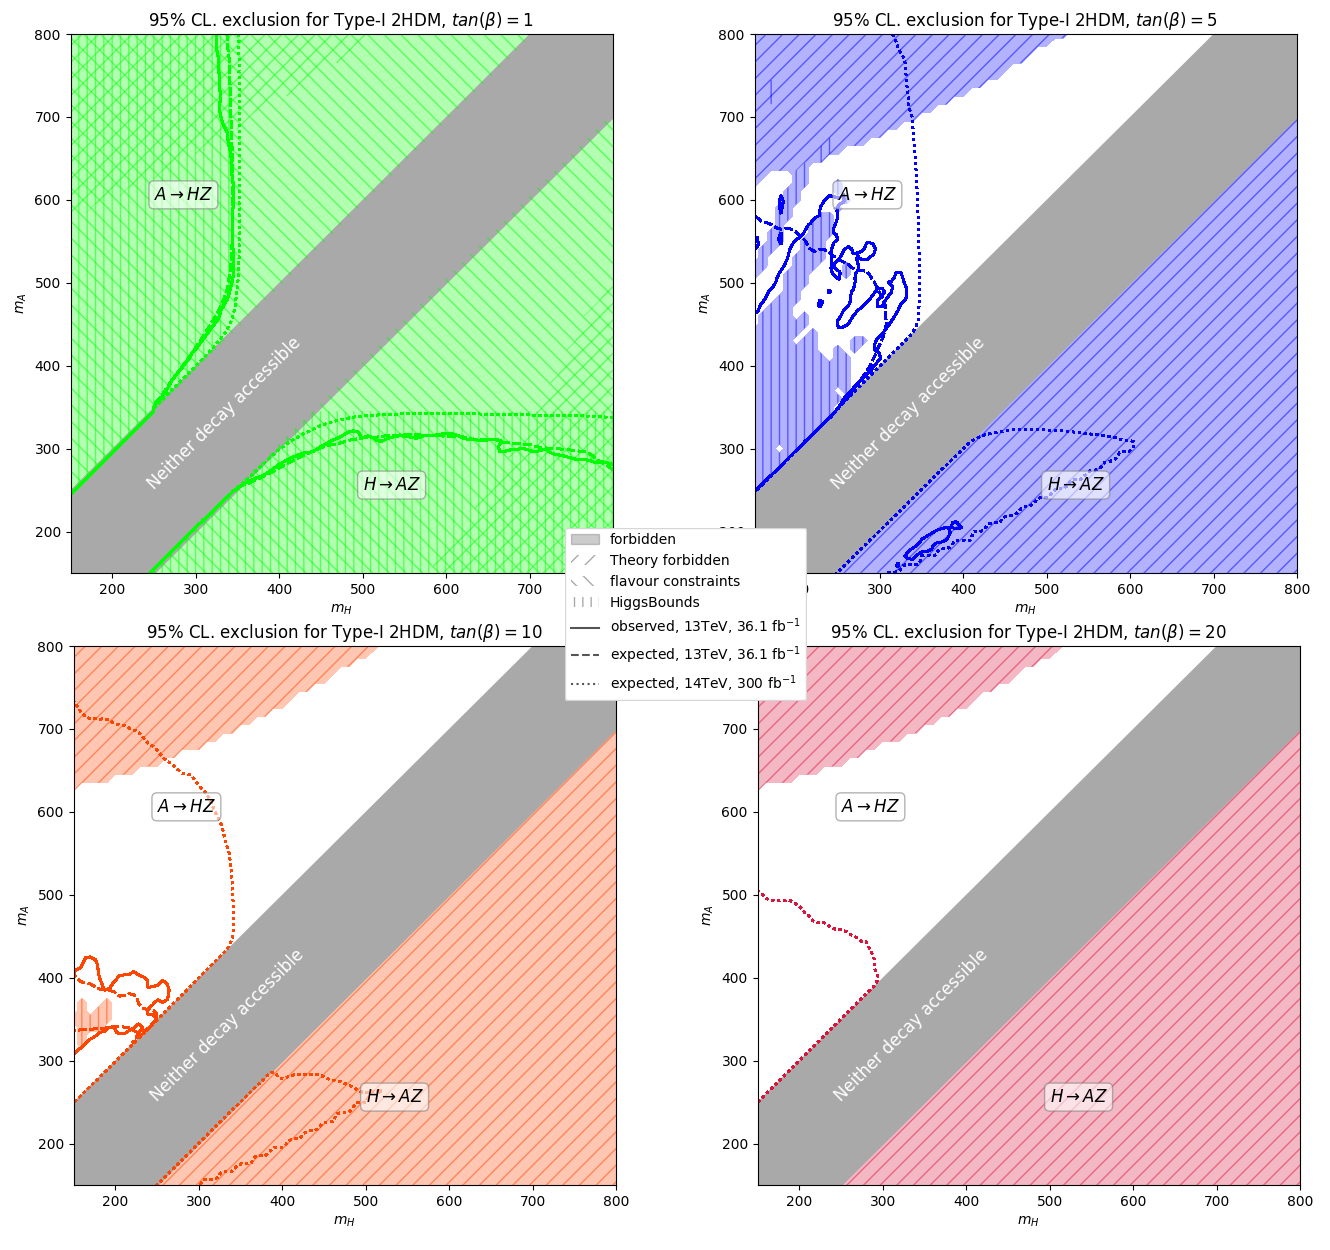
\includegraphics[width=\textwidth]{single_tbs/type1.png}
    \caption{Exclusion limits at \(95\%\) CL in Type-I.
             The lines denoting expected and observed exclusion limits
             do not appear at all on some plots when the prediction never exceeds the 
             expected or observed  limit.}\label{fig1}
\end{figure}

\begin{figure}[t!]		
    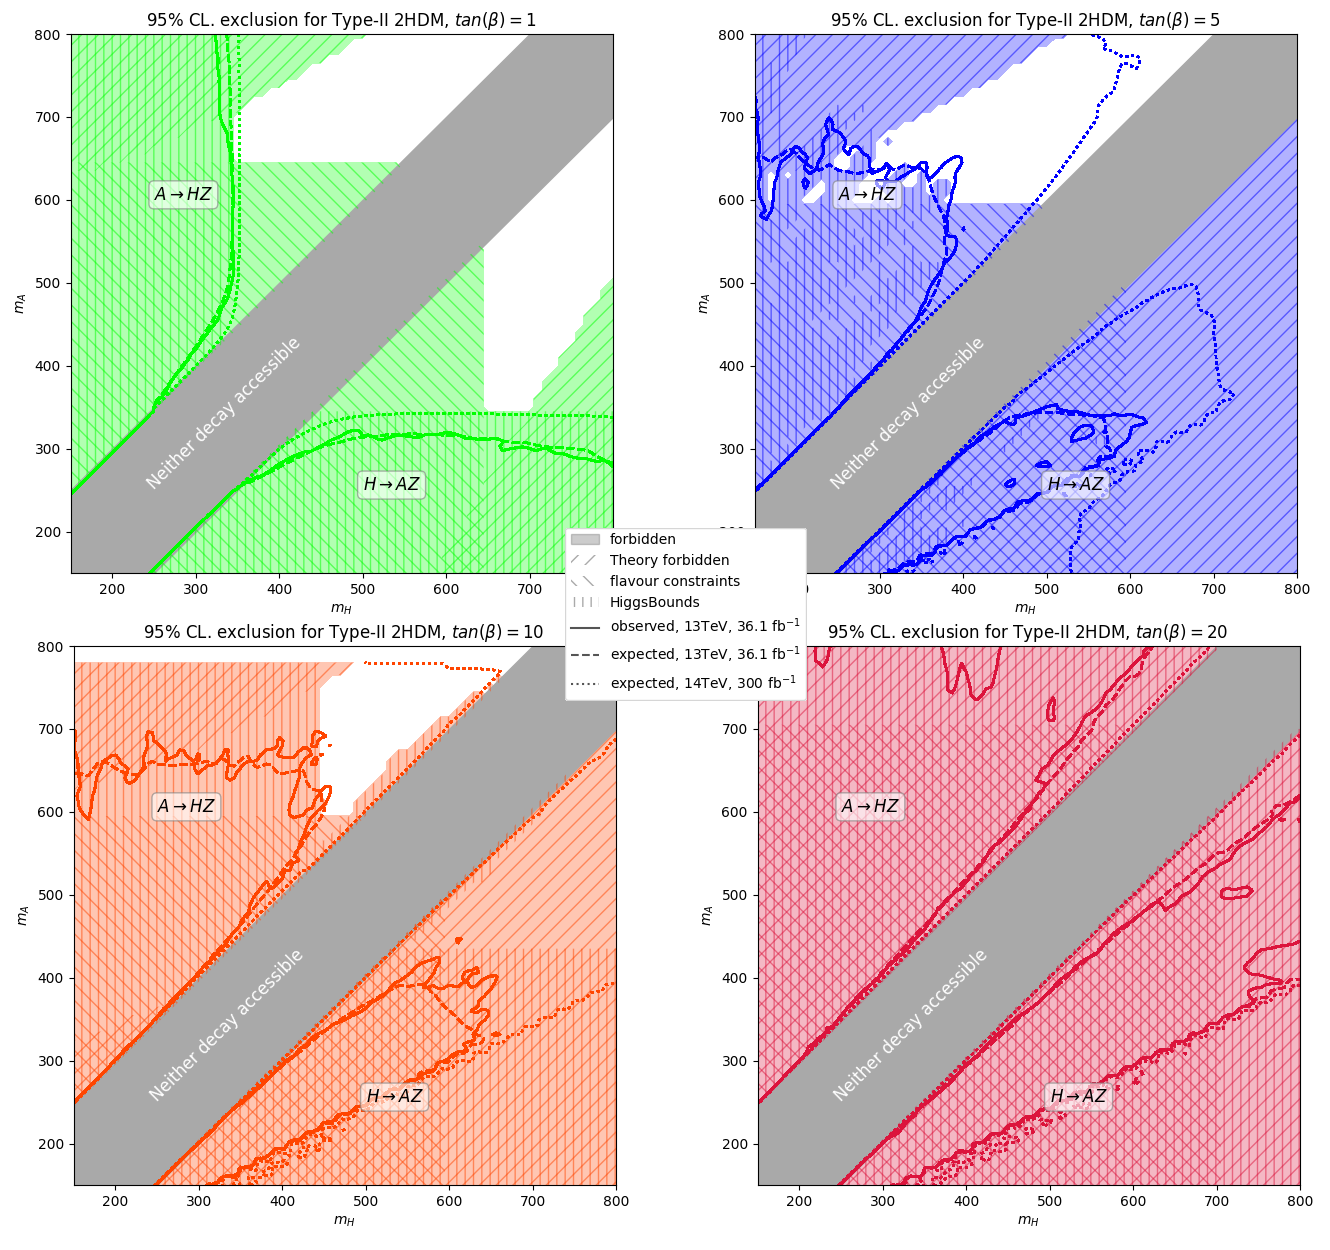
\includegraphics[width=\textwidth]{single_tbs/type2.png}
    \caption{Like in Fig.~\ref{fig1} but for Type-II.}\label{fig2}
\end{figure}


\begin{figure*}[t!]	     
    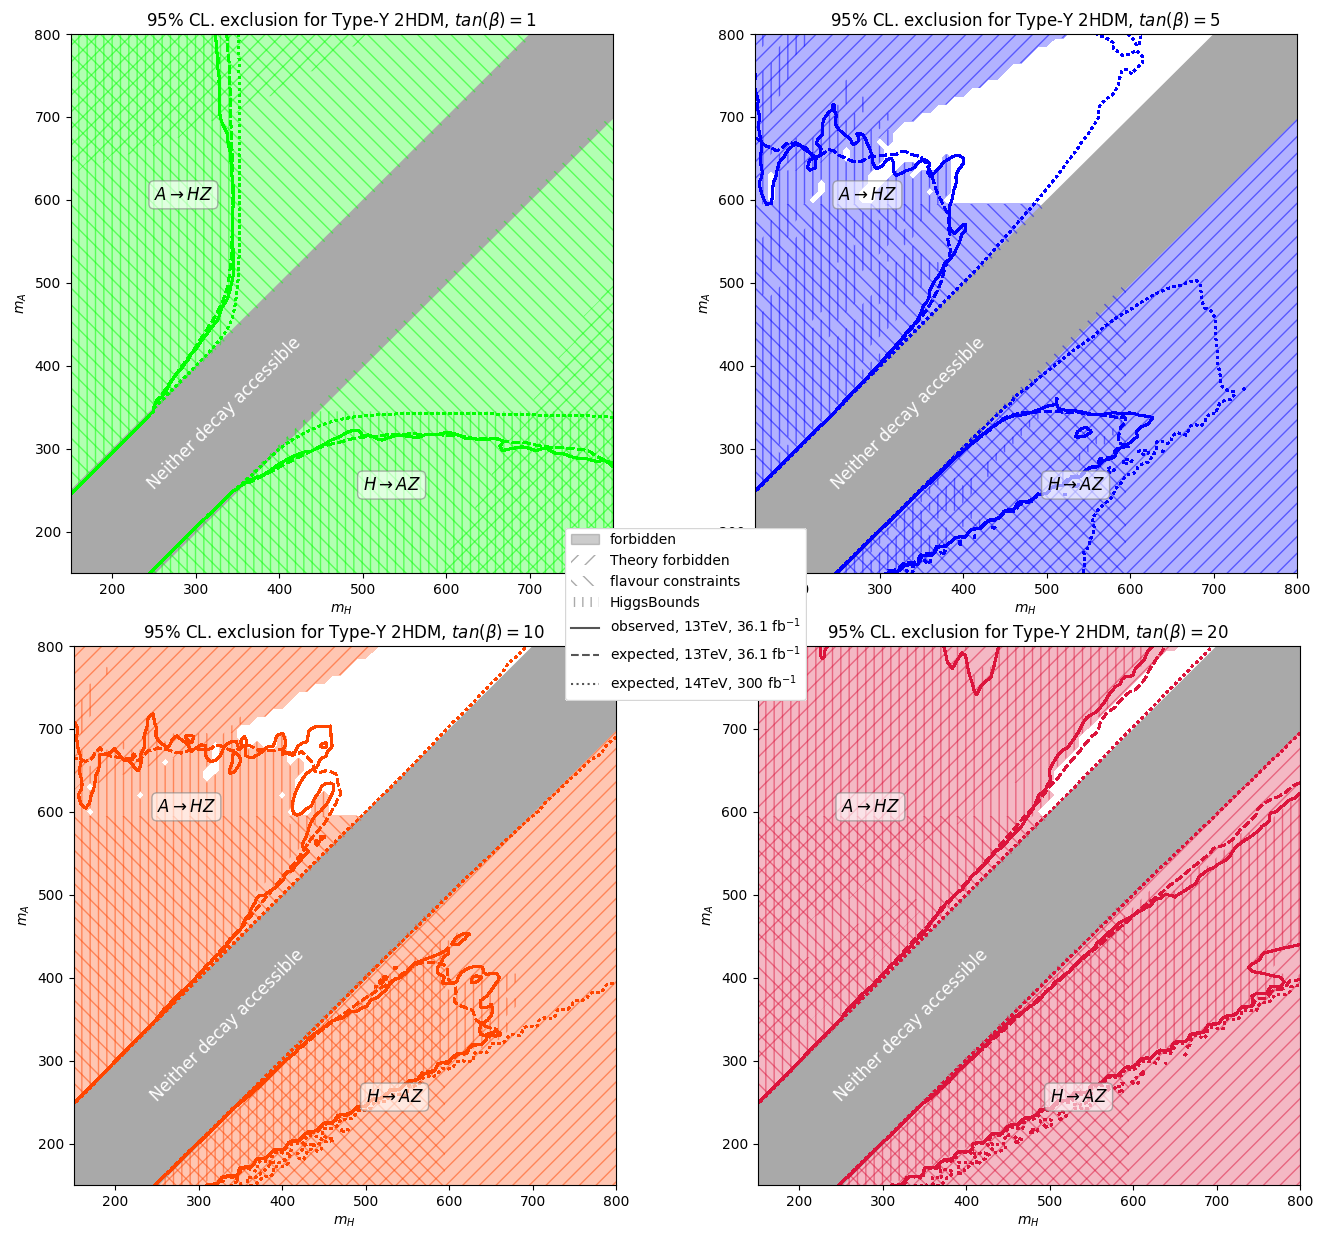
\includegraphics[width=\textwidth]{single_tbs/type3.png}
    \caption{Like in Fig.~\ref{fig1} but for Type-Y (Flipped).}\label{fig3}
\end{figure*}

\begin{figure*}[t!]
	\centering
    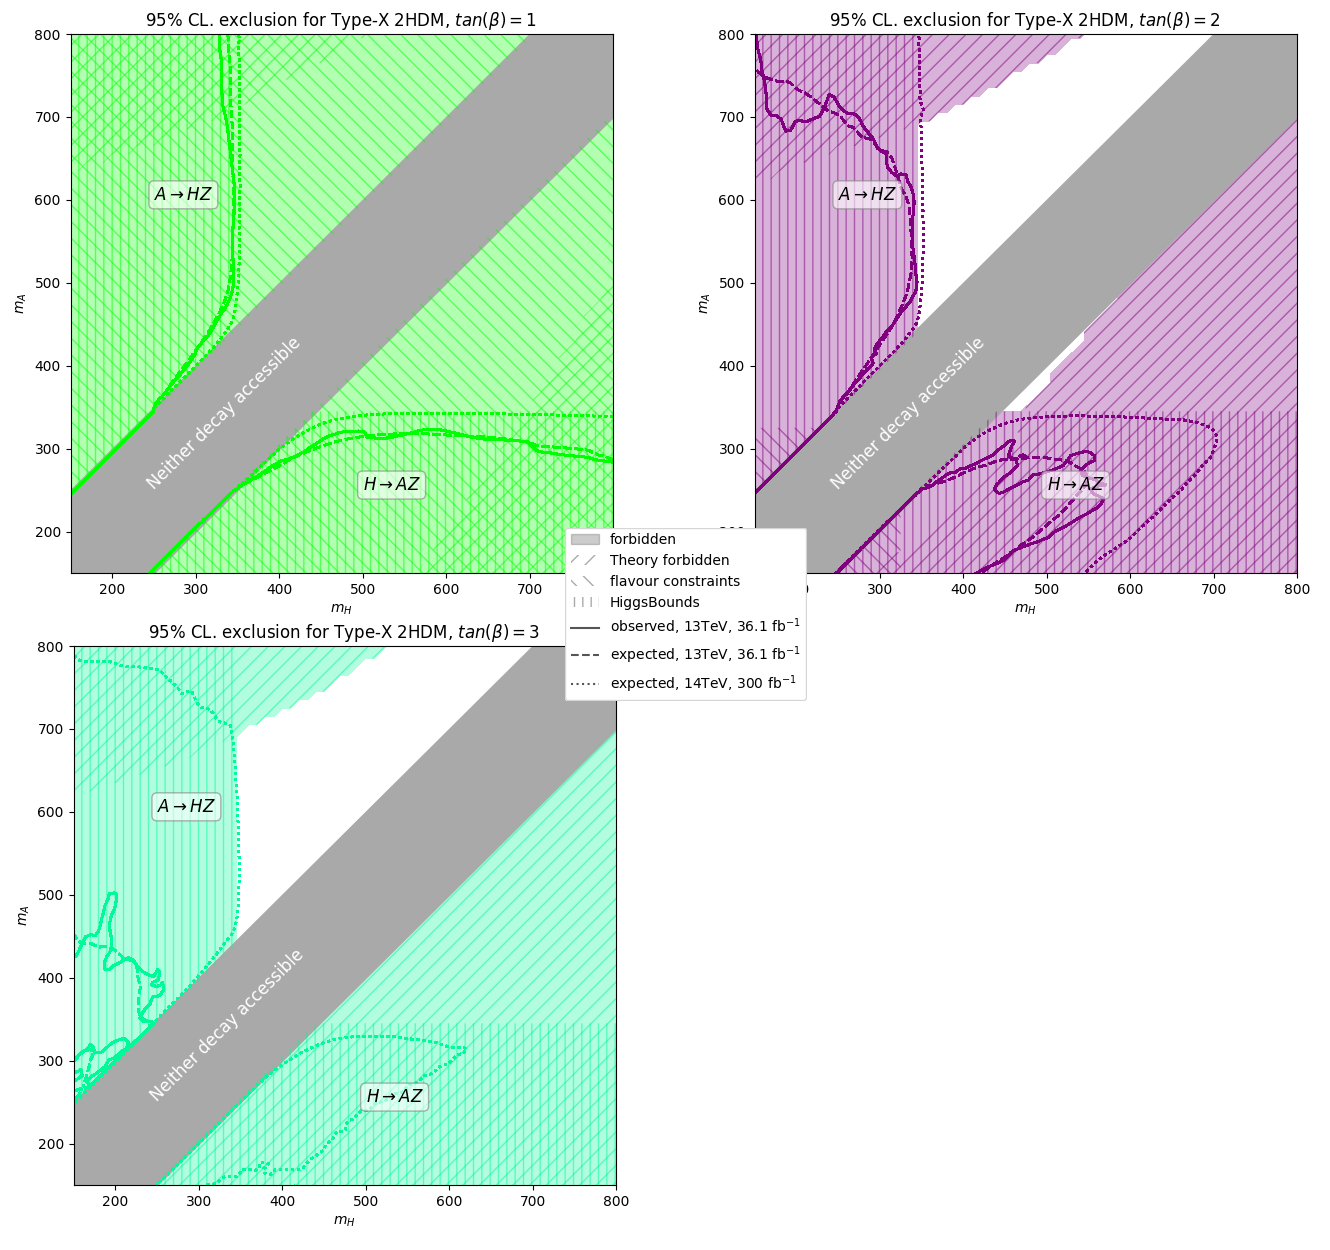
\includegraphics[width=\textwidth]{single_tbs/type4.png}
    \caption{Like in Fig.~\ref{fig1} but for  Type-X (Lepton specific).}\label{fig4}
\end{figure*}


\begin{figure*}[t!]
	\centering
    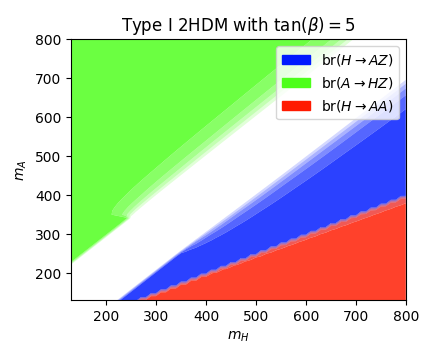
\includegraphics[width=.5\textwidth]{branching_ratios_HAA.png}
    \caption{The branching ratio \(H\rightarrow AZ\) is suppressed by the branching ratio \(H\rightarrow AA\).
             This effect occurs for all types, but does not occur at small \(\tan(\beta)\).}\label{figsuppress}
\end{figure*}


\begin{table}
\begin{tabularx}{\textwidth}{RCCCC}
      \toprule
      \textcolor{black}{\(\tan(\beta)\)}& \textcolor{black}{\(1\)} & \textcolor{black}{\(5\)} & \textcolor{black}{\(10\)} & \textcolor{black}{\(20\)}\\
      \toprule
      Type-I & \textcolor{red}{Flavour constraints} & \textcolor{blue}{Some masses} & \textcolor{blue}{Many masses} & \textcolor{red}{Low sensitivity} \\
      \hline
      Type-II &\textcolor{red}{Flavour constraints} & \textcolor{blue}{Some masses after upgrade} & \textcolor{blue}{Some masses after upgrade} & \textcolor{red}{Theory constraints}\\
      \hline
      Flipped &\textcolor{red}{Flavour constraints} & \textcolor{blue}{Some masses after upgrade} & \textcolor{blue}{Some masses after upgrade} & \textcolor{red}{Theory constraints}\\
      \toprule
      \textcolor{black}{\(\tan(\beta)\)}& \textcolor{black}{\(1\)} & \textcolor{black}{\(2\)} & \textcolor{black}{\(3\)} & \\
      \toprule
      Lepton specific & \textcolor{red}{Flavour constraints} & \textcolor{red}{Excluded by HiggsBounds} &  \textcolor{red}{Excluded by HiggsBounds} & \\
\end{tabularx}
%\vspace*{-1cm}
\caption{Table summarising the findings in Figs.~\ref{fig1}~to~\ref{fig4}.
An overview of the possibility of each Yukawa type and value of \(\tan(\beta)\) is given.
Entries in red indicate that the combination has little or no mass combinations that are not forbidden while those in blue represent available parameter space accessible presently at Run 2  or after the upgrade of Run 3.}
\label{tab:summary}
\end{table}

After performing a scan over the parameter space delimited by Eq.~(\ref{eq1}), we compare the prediction of the model with the observed and expected limits given in Ref.~\cite{Aaboud2018AZHbbll}.
If the prediction exceeds the observed limit, then the parameter combination is excluded.
When the prediction exceeds the expected limit, we anticipate that the signal would be visible above background given the energies and luminosities available, hence,  {the experiment is sensitive to these parameters.} %these parameters are testable.



The choice of \(m^2_{12} = m_A^2 \tan(\beta) / (1 + \tan(\beta))^2\) enables us to reconstruct the exclusion limits at 95\%  CL given in Ref~\cite{Aaboud2018AZHbbll}.
However, this choice does not actually allow to satisfy theoretical constraints in all four types of 2HDM.
Therefore, we have dismissed it in our analysis.
In contrast, our choice of \(m_{12}^2\) above aims to simultaneously satisfy as many theoretical constraints as possible while affording one with significant parameter space amenable to experimental investigation.
Indeed, this is achieved by randomly sampling values of \(m^2_{12}\) between \(0\) and \(2\times 10^{5}\)~GeV for each point of the scan and selecting the one that passes most theoretical checks.



Figs.~\ref{fig1}~to~\ref{fig4} illustrate the outcome the scan for each
Yukawa type, \(\tan(\beta)\) and mass combination $(m_H,m_A)$.
Each figure provides results for one choice of Yukawa couplings
and each frame in each figure provides results at one value of \(\tan(\beta)\).
In the top left of each plot, where \(m_A > m_H+100\)~GeV, the decay \AZH{} is considered while 
in the bottom right of each plot, where \(m_H > m_A+100\)~GeV,   the decay \HZA{} is considered.
The corridor along the diagonal between these regions is coloured grey to indicate that neither decay is accessible.
%
If a combination of parameters is forbidden by theory, HiggsBounds or flavour constraints
then the corresponding area is filled with solid colour, conversely,
white areas pass all these checks and so are of interest. The hatching over the solid colour is used to indicate which of the checks
causes the corresponding parameter combination to fail.
There are three boundary lines drawn over the plots: 
these are the observed and expected \(95\%\) CLs for the ATLAS detector in its present state, \(13\) TeV and \(36.1~\text{fb}^{-1}\),
plus the expected 95\% CL for an upgraded LHC and ATLAS detector at \(14\) TeV and \(300~\text{fb}^{-1}\)\footnote{We neglect here to consider the case of $\sqrt s=13$ TeV and $L\approx140$ fb$^{-1}$, as it only improves marginally the present situation yet it would be make the plots far too crowded.}.
The model predictions exceed the 95\% CL inside the curve.

In Fig.~\ref{fig1} the parameter space with Type-I Yukawa couplings is shown.
The upper left plot shows that \(\tan(\beta) = 1\) is always forbidden by flavour constraints.
The upper right plot shows that there are many mass combinations that do not prevent the decay \AZH{} for \(\tan(\beta) = 5\),
but theory constraints forbid all mass combinations relevant to \HZA{}.
At \(\tan(\beta) = 5\) for \(13\) TeV (and \(36.1~\text{fb}^{-1}\)) the area of sensitivity (inside the expected curve) that is not excluded by observation (inside the observed curve) is very limited. 
\textcolor{red}{It is also seen that the \(H\rightarrow AZ\) signal has reduced sensitivity when \(\tan(\beta)\) is \(5\) or more.
This is due to \(H\rightarrow AA\) competing with \(H\rightarrow AZ\), as shown in figure~\ref{figsuppress}.
The branching ratio \(H\rightarrow AA\) becomes significant because of the enhancement of the trilinear coupling \(\lambda_{HAA}\) at large \(\tan(\beta)\).}
At \(14\) TeV and \(300~\text{fb}^{-1}\), however, we expect many mass combinations to be testable that have not yet been excluded.
The lower left plot shows the behaviour at \(\tan(\beta) = 10\) to be similar to \(\tan(\beta) = 5\), i.e., 
everything is forbidden for \HZA{} by theory while for \AZH{} most combinations for which there is sensitivity have been excluded at \(13\) TeV
but \(14\) TeV offers even more possible parameter space than seen at \(\tan(\beta) = 5\).
Finally, in the lower right frame of Fig.~\ref{fig1}, the parameter space for \(\tan(\beta) = 20\) is shown.
The state of \HZA{} is unchanged, but now \AZH{} has no expected or observed exclusion at \(13\) TeV, i.e., these parameters are harder to probe.
With the upgrade to \(14\) TeV and 300 fb$^{-1}$ there is some sensitivity to \AZH{} at \(\tan(\beta) = 20\).

As might be expected, the behaviour of Type-II, shown in Fig.~\ref{fig2} and Type-Y, shown in Fig.~\ref{fig3}, is remarkably similar.
The upper left plot shows that \(\tan(\beta) = 1\) is forbidden by flavour constraints in all areas where there is sensitivity.
At \(13\) TeV  and 36.1 fb$^{-1}$ the upper right plot shows that the same can be said for \(\tan(\beta) = 5\), however,
after Run 3,  at \(14\) TeV and 300 fb$^{-1}$, there are many permitted mass combinations for \AZH{}. However, 
\HZA{} is excluded by theory.
The behaviour at \(\tan(\beta) = 10\), shown in the lower left plot, is much the same as for \(\tan(\beta) = 5\),
except more of the exclusion at \(13\) TeV and 36.1 fb$^{-1}$  is from observations provided by HiggsBounds.
Finally, in the lower right plot, \(\tan(\beta) = 20\) is shown to be excluded for almost all mass choices,
by multiple constraints.

In Fig.~\ref{fig4} the behaviour of the Type-X 2HDM is shown, at a set of \(\tan(\beta)\) values that differs from those previously considered.
\textcolor{red}{The change is made because the parameter space in Type-X shrinks more rapidly with increasing \(\tan(\beta)\) compared to the other Yukawa types.}
For these choices HiggsBounds excludes all areas inside the expected limits.
This remains true even after the end of Run 3.

Finally, Tab.~\ref{tab:summary} summarises our findings, highlighting that sensitivity only really exists for $5<\tan(\beta)<10$ and limitedly to the 2HDM Type-I, both at Run 2 and 3, and -II and -Y (or Flipped), but only at Run 3. The case of Type-X (or Lepton specific) is never accessible.


\subsection{Conclusions}
In summary, we have revisited an experimental analysis of the ATLAS Collaboration of the production and decay process $gg,b\bar b\to A\to ZH\to l^+l^-b\bar b$ performed at Run 2 with 36.1 fb$^{-1}$ of luminosity, which had been interpreted in terms of exclusion limits over the parameter space of the four types of the 2HDM, wherein the lightest Higgs state is identified with the SM-like Higgs boson discovered during Run 1 at the LHC with mass 125 GeV. Upon validating the ATLAS interpretation in our framework, though, we have discovered that their (fixed) choice of $m_{12}$, a mass parameter in the 2HDM Lagrangian that softly breaks an underlying $Z_2$ symmetry of the 2HDM to avoid FCNCs, yields parameter space configurations which are ruled out by theoretical requirements of model consistency. Hence, we have allowed this parameter to vary freely and subject the ensuing parameter space configurations to both the aforementioned theoretical constraints as well as those emerging from past and present experiments, thereby redrawing the actual sensitivity of such an experimental search to all four Yukawa types of the 2HDM, as a function of $\tan(\beta)$. In doing so, we have have also forecast the potential sensitivity of this channel to the 2HDM parameter space at the end of Run 3, assuming increased energy to 14 TeV and luminosity to 300 fb$^{-1}$.
This revealed some extended coverage of the 2HDM Type-I, -II and -Y (but not -X), %{\textcolor{red}{SM: the previous sentence might need revising once the mixup with Figs. 2--4 is fixed}} Henry: fixed.
especially for intermediate $\tan(\beta)$ values (say, between  5 and 10), with $m_A$ up to 800 GeV and $m_H$ up to 700 GeV.
This is somewhat beyond what is presently covered, i.e.,  up to 150 GeV or so in mass of either Higgs state, so as to justify further searches for this signature at the next stage of the LHC. Finally, we have recast the sensitivity of this analysis onto that of the channel  $gg,b\bar b\to H\to ZA\to l^+l^-b\bar b$. However, we have found that the complementary parameter space accessible this way (i.e., $m_H\ge  m_A+m_Z$) is actually entirely excluded already by existing theoretical and/or experimental constraints, so as to conclude that it is not warranted to pursue further this channel at the LHC, at least, not with a view to interpret it in the context of the standard four Yukawa types of the 2HDM\footnote{We finally note that analyses similar to Ref.~\cite{Aaboud2018AZHbbll}
performed by the CMS Collaboration exist \cite{Khachatryan2016resonancesbbtautau,Sirunyan2020newneutral}. We have not used these for two reasons. On the one hand, they did not convey all the  information necessary to make  extrapolations to higher energies. On the other hand, they did not afford one with significantly different sensitivity to the 2HDM at present energies than what achieved by the ATLAS analysis ~\cite{Aaboud2018AZHbbll} that we have adopted as benchmark.}.

